\documentclass[a4paper, 12pt]{article}
\usepackage{fullpage}

\usepackage{amsmath}
\usepackage{amssymb}
\usepackage{amsfonts}
\usepackage{amsthm}
\usepackage{mathtools}
\usepackage{soul}
\usepackage{hyperref}

\usepackage{color}
\usepackage{listings}

\definecolor{mygreen}{rgb}{0.0, 0.5, 0.0}
\definecolor{emphamber}{rgb}{1.0, 0.75, 0.0}
\definecolor{amber}{rgb}{1.0, 0.49, 0.0}
\definecolor{ballblue}{rgb}{0.13, 0.67, 0.8}
\definecolor{gray}{rgb}{0.5, 0.5, 0.5}

\lstdefinestyle{kamyarStyle}{
    basicstyle=\footnotesize\ttfamily,
    keywordstyle=\color{amber},
    stringstyle=\color{mygreen},
    commentstyle=\color{gray},
    breakatwhitespace=false,
    breaklines=true,
    keepspaces=true,
    showspaces=false,
    showstringspaces=false,
    showtabs=false,
}

\lstset{style=kamyarStyle}
\lstset{escapeinside={(*@}{@*)}}

\hypersetup{colorlinks=true, urlcolor=cyan}

\usepackage{xepersian}

\settextfont{XB Zar}
\ExplSyntaxOn \cs_set_eq:NN \etex_iffontchar:D \tex_iffontchar:D \ExplSyntaxOff
\setmathdigitfont{Yas}

\renewcommand{\baselinestretch}{1.3}

\begin{document}

\textbf{حسابگری زیستی؛}

\textbf{یافتن کمینه و بیشینه توابع ریاضی به کمک روش بهینه‌سازی ازدحام ذرات؛}

\textbf{کامیار میرزاوزیری؛ 610396152}

\hrulefill

\section{مقدمات و ابزارها}

\subsection{ترسیم‌گر}
کلاسی به اسم
\texttt{Visualizer}
پیاده‌سازی می‌کنیم که وظیفه ترسیم توابع و ذرات را دارد. این کلاس از کتابخانه
\texttt{matplotlib}
برای ترسیم استفاده می‌کند و کد آن در فایل
\texttt{utils.py}
موجود است اما چون مربوط به موضوع پروژه نمی‌باشد به آن نمی‌پردازیم.

\subsection{ذره}
کلاسی به اسم
\texttt{Particle}
به نمایندگی از ذرات ایجاد می‌کنیم که هر
\texttt{instance}
آن نماینده یک ذره باشد. هر ذره باید مختصات فعلی خود یعنی
\texttt{x}
و
\texttt{y}
را به خاطر داشته باشد و محاسبه مقدار تابع یعنی
\texttt{z}
با داشتن این مقادیر امکان‌پذیر است اما برای تسریع الگوریتم این مقدار را نیز در اشیاء نگه می‌داریم. همچنین هر ذره باید بهترین وضعیتی که تا کنون داشته را به خاطر داشته باشد، و به پارامترهایی نظیر
$\omega$
و
$c_i$
نیز دسترسی داشته باشد. پس
\texttt{constructor}
این کلاس را به صورت زیر پیاده‌سازی می‌کنیم.

\LTR
\begin{lstlisting}[language=Python]
def __init__(self, x, y, func, x_range, y_range, better, omega, c_1, c_2, c_3, t, cooling_ratio):
    self.func = func
    self.x_range = x_range
    self.y_range = y_range
    self.better = better
    self.omega = omega
    self.c_1 = c_1
    self.c_2 = c_2
    self.c_3 = c_3
    self.t = t
    self.cooling_ratio = cooling_ratio
    self.x = x
    self.y = y
    self.z = self.func(self.x, self.y)
    self.best = (self.x, self.y, self.z)
    self.v_x = 0
    self.v_y = 0
\end{lstlisting}
\RTL

\begin{itemize}
    \item پارامتر
          \texttt{x}
          نشان‌دهنده مختصات ذره در محور
          $x$ها
          می‌باشد.
    \item پارامتر
          \texttt{y}
          نشان‌دهنده مختصات ذره در محور
          $y$ها
          می‌باشد.
    \item پارامتر
          \texttt{func}
          تابعی است که
          $z$
          بر اساس آن از روی
          $x$
          و
          $y$
          محاسبه می‌شود و می‌تواند
          $f$
          یا
          $g$
          باشد.
    \item پارامتر
          \texttt{x\_range}
          یک لیست دوتایی شامل حداقل و حداکثر مقدار
          $x$
          است که در تابع
          $f$
          مقادیر
          $[-10, 10]$
          و در
          $g$
          مقادیر
          $[-100, 100]$
          را دارد.
    \item پارامتر
          \texttt{y\_range}
          مشابه
          \texttt{x\_range}
          اما برای
          $y$
          می‌باشد.
    \item پارامتر
          \texttt{better}
          تابعی با دو ورودی می‌باشد که اگر ورودی اول بهتر از دوم باشد
          \texttt{True}
          برمی‌گرداند. برای
          $f$
          که به دنبال ماکسیمم هستیم این تابع باید بزرگ‌تری باشد و برای
          $g$
          کوچک‌تری.
    \item پارامترهای
          \texttt{omega}،
          \texttt{c\_1}
          و
          \texttt{c\_2}
          همان پارامترهای الگوریتم
          \texttt{PSO}
          می‌باشند.
    \item برای پارامتر
          \texttt{c\_3}
          لازم است اشاره کنیم که در این تمرین تصمیم گرفتیم تا برای آزمایش مقداری نویز به ذرات اضافه کنیم تا قابلیت پویش را بالا ببریم. به این صورت که در هر تکرار الگوریتم در زمان تعیین سرعت، عددی تصادفی را نیز به سرعت اضافه می‌کنیم که می‌تواند مثبت یا منفی باشد و این عدد در ضریب
          \texttt{c\_3}
          ضرب شده و نتیجه به بردار سرعت اضافه می‌شود.
    \item پارامتر
          \texttt{t}
          برای کنترل نویز به کار می‌رود. نویزی که توضیح دادیم را به کمک الگوریتم تبرید تدریجی کنترل می‌کنیم پس نیاز به پارامتری به عنوان دمای اولیه داریم.
    \item پارامتر
          \texttt{cooling\_ratio}
          مربوط به همان الگوریتم تبرید تدریجی نویز ذرات می‌باشد.
\end{itemize}

در هر تکرار الگوریتم
\texttt{PSO}
لازم است ذره را بروزرسانی کنیم. برای این منظور متد
\texttt{update}
را روی کلاس ذره تعریف می‌کنیم. در این کلاس ابتدا بررسی می‌کنیم و اگر ذره‌ای در نقطه بهینه سراسری قرار داشت آن را حرکت نمی‌دهیم تا از از دست دادن بهینه سراسری جلوگیری کنیم و به قابلیت انتفاع کمک کنیم. اما اگر چنین نبود بردار سرعت را مطابق با روش
\texttt{PSO}
و افزودن نویز محاسبه می‌کنیم و سپس مکان جدید ذره را محاسبه می‌کنیم. در این مرحله امکان دارد ذره از محدوده مقادیر معتبر خود خارج شود. در این صورت بردار سرعت آن را منفی می‌کنیم و دوباره روی آن اثر می‌دهیم (مشابه اثری که برخورد با دیواره برای یک ذره دارد و باعث می‌شود در جهت عکس بازگردد)، اما اگر بردار سرعت بزرگ بود و در جهت عکس هم از محدوده خارج می‌شد ناچاریم آن را در انتهای محدوده قرار دهیم. در نهایت مقدار
\texttt{z}
را بر اساس
\texttt{x}
و
\texttt{y}
جدید محاسبه کرده و در صورتی که از بهترین خود ذره بهتر بود آن را جایگزین می‌کنیم.
\newpage
\LTR
\begin{lstlisting}[language=Python]
def update(self, global_best):
    self.t *= self.cooling_ratio
    if self.z == global_best[2]:
        return

    self.v_x = (
        self.omega * self.v_x +
        self.c_1 * random() * (self.best[0] - self.x) +
        self.c_2 * random() * (global_best[0] - self.x) +
        self.c_3 * self.t * (.5 - random())
    )
    self.v_y = (
        self.omega * self.v_y +
        self.c_1 * random() * (self.best[1] - self.y) +
        self.c_2 * random() * (global_best[1] - self.y) +
        self.c_3 * self.t * (.5 - random())
    )

    new_x = self.x + self.v_x
    if new_x < self.x_range[0] or new_x > self.x_range[1]:
        self.v_x *= -.5
    self.x += self.v_x
    self.x = min(max(self.x, self.x_range[0]), self.x_range[1])

    new_y = self.y + self.v_y
    if new_y < self.y_range[0] or new_y > self.y_range[1]:
        self.v_y *= -.5
    self.y += self.v_y
    self.y = min(max(self.y, self.y_range[0]), self.y_range[1])

    self.z = self.func(self.x, self.y)
    if self.better(self.z, self.best[2]):
        self.best = (self.x, self.y, self.z)
\end{lstlisting}
\RTL

\newpage
\section{ازدحام}
کلاس
\texttt{Swarm}
را به نمایندگی از ازدحام ذرات پیاده‌سازی می‌کنیم. در
\texttt{constructor}
این کلاس نیز مشابه کلاس ذره تعدادی پارامتر دریافت می‌کنیم.
\LTR
\begin{lstlisting}[language=Python]
def __init__(self, func, x_range, y_range, iterations_count, visualizer, better, best, sqrt_count, omega, c_1, c_2, c_3, t, cooling_ratio):
    self.func = func
    self.x_range = x_range
    self.y_range = y_range
    self.iterations_count = iterations_count
    self.visualizer = visualizer
    self.better = better
    self.best = best
    self.count = sqrt_count ** 2
    self.omega = omega
    self.c_1 = c_1
    self.c_2 = c_2
    self.c_3 = c_3
    self.t = t
    self.cooling_ratio = cooling_ratio

    self.particles = []
    for x in np.linspace(x_range[0] + .1, x_range[1] - .1, sqrt_count):
        for y in np.linspace(y_range[0] + .1, y_range[1] - .1, sqrt_count):
            self.particles.append(Particle(
                x + (.5 - random()) / 5, y + (.5 - random()) / 5,
                func, x_range, y_range, better, omega, c_1, c_2, c_3, t, cooling_ratio
            ))
\end{lstlisting}
\RTL

\begin{itemize}
    \item پارامتر
          \texttt{iterations\_count}
          تعداد تکرارهای الگوریتم را نشان می‌دهد. در این تمرین شرط توقف را تعداد در نظر گرفتیم.
    \item پارامتر
          \texttt{visualizer}
          یک ترسیم‌کننده در اختیار ازدحام قرار می‌دهد تا بتواند تابع و ذرات را در فضای سه‌بعدی رسم کند.
    \item پارامتر
          \texttt{best}
          مشابه پارامتر
          \texttt{better}
          که در بخش قبل توضیح دادیم یک تابع است که با دریافت لیستی از نقاط بهترین را خروجی می‌دهد. این تابع برای
          $f$
          برابر
          \texttt{max}
          و برای
          $g$
          برابر
          \texttt{min}
          می‌باشد.
    \item پارامتر
          \texttt{sqrt\_count}
          نشان‌دهنده ریشه دوم تعداد ذرات می‌باشد. علت این است که در این تمرین تصمیم گرفتیم به جای انتخاب تصادفی ذرات، آن‌ها به طور کاملا منظم و با فواصل برابر از محدوده مجاز انتخاب کنیم. پس برای مثال اگر این پارامتر برابر
          $10$
          باشد، محدوده مجاز برای
          $x$ها
          را به
          $10$
          و
          $y$ها
          را نیز به
          $10$
          قسمت تقسیم می‌کنیم و از این طریق
          $100$
          نقطه انتخاب می‌کنیم و ذرات را ایجاد می‌کنیم.
\end{itemize}

در نهایت برای اجرای الگوریتم کافی است مطابق آنچه در کلاس بیان شده پیش برویم.

\LTR
\begin{lstlisting}[language=Python]
def run(self, printing_iterations=[], visualizing_iterations=[], output=None):
    for iteration in range(self.iterations_count + 1):
        values = [particle.z for particle in self.particles]
        global_best_index = values.index(self.best(values))
        global_best = (self.particles[global_best_index].x,
                        self.particles[global_best_index].y, self.particles[global_best_index].z)

        if iteration in printing_iterations:
            print(f'Iteration: {iteration}\tBest: {global_best}')
        if iteration in visualizing_iterations:
            self.visualizer.add(self.x_range, self.y_range, self.func, self.particles,
                                title=f'Iteration {iteration}\nBest: {round(global_best[2], 2)}')

        for particle in self.particles:
            particle.update(global_best)

    self.visualizer.show(output)
\end{lstlisting}
\RTL

در این قطعه کد نکته خاصی وجود ندارد، تنها مراحل ساده
\texttt{PSO}
پیاده‌سازی شده‌اند.

\newpage

\section{نتایج}

\subsection{تابع $f$}
برای این تابع قطعه کد زیر را نوشتیم

\LTR
\lstinputlisting[language=Python]{f.py}
\RTL

برای رسیدن به پاسخ مورد نظر ۲۰ تکرار روی ۱۶۰۰ ذره انجام دادیم، که نتیجه زیر حاصل شد.

\LTR
\lstinputlisting{results/f.out.txt}
\RTL

که از چیزی که در تمرین خواسته شده بهتر است.

\begin{center}
    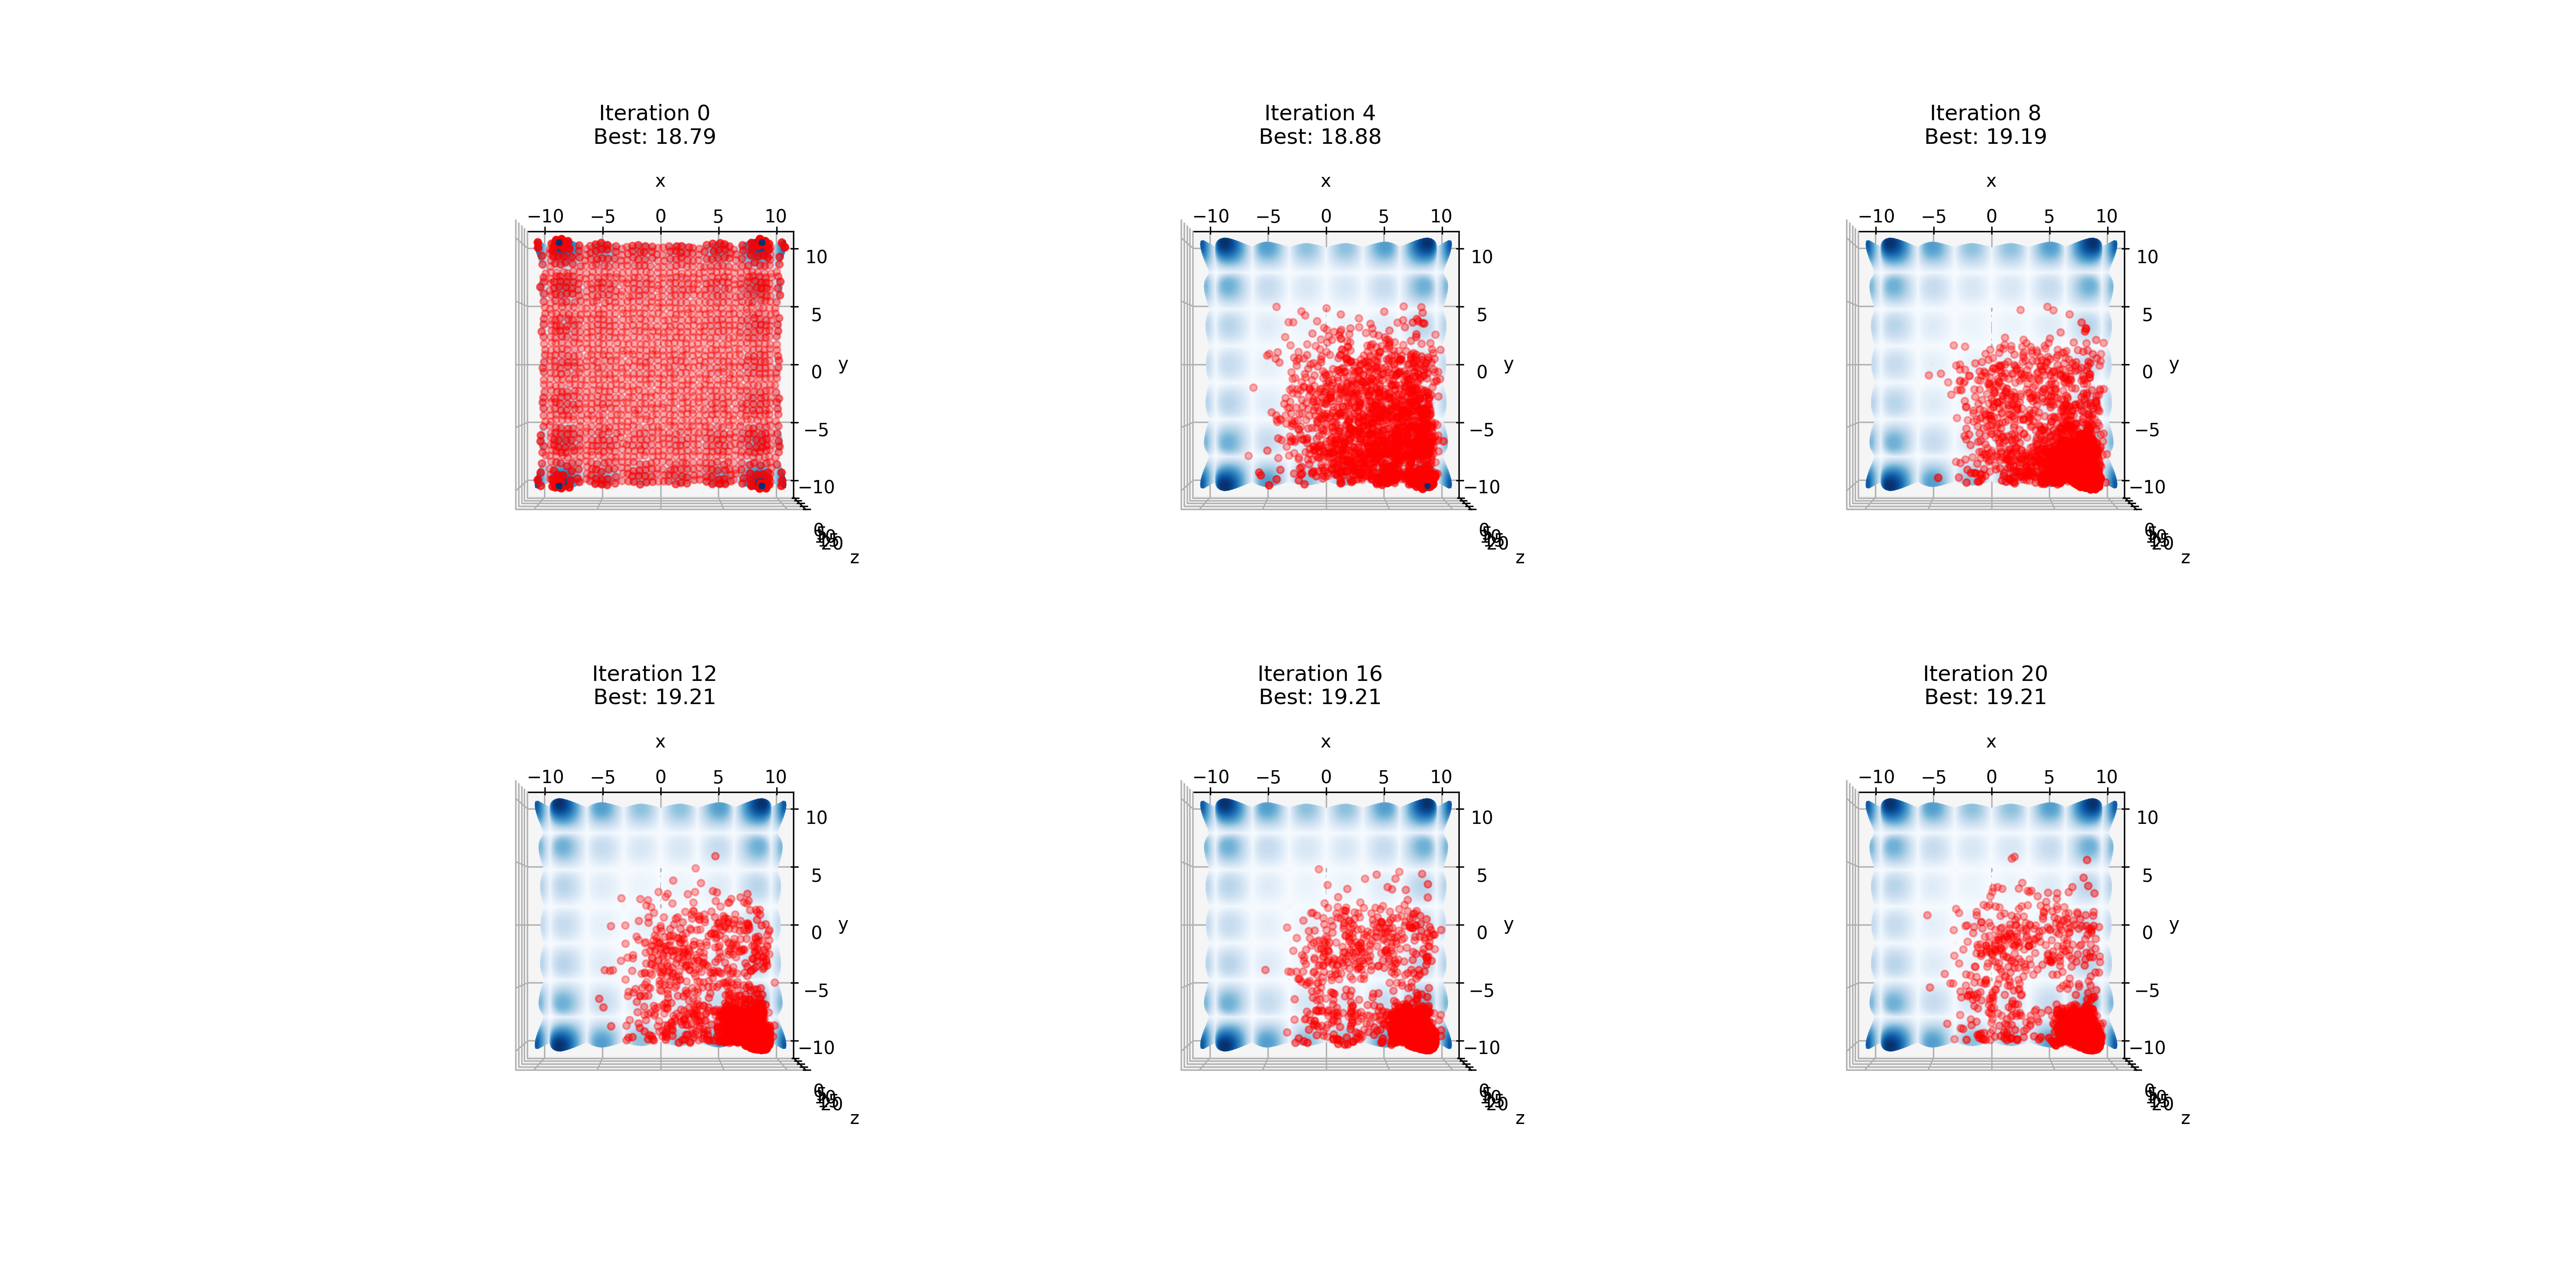
\includegraphics[width=1\textwidth]{results/f.png}
\end{center}

این تصاویر از زاویه بالا رسم شده‌اند.

\newpage
\subsection{تابع $g$}
برای این تابع کار کمی سنگین‌تر شد. قطعه کد زیر را نوشتیم

\LTR
\lstinputlisting[language=Python]{g.py}
\RTL

برای رسیدن به پاسخ مورد نظر ۴۰۰۰ تکرار روی ۱۶۰۰ ذره انجام دادیم، که نتیجه زیر حاصل شد.

\LTR
\lstinputlisting{results/g.out.txt}
\RTL

که با اختلاف از چیزی که در تمرین خواسته شده بهتر است.

\begin{center}
    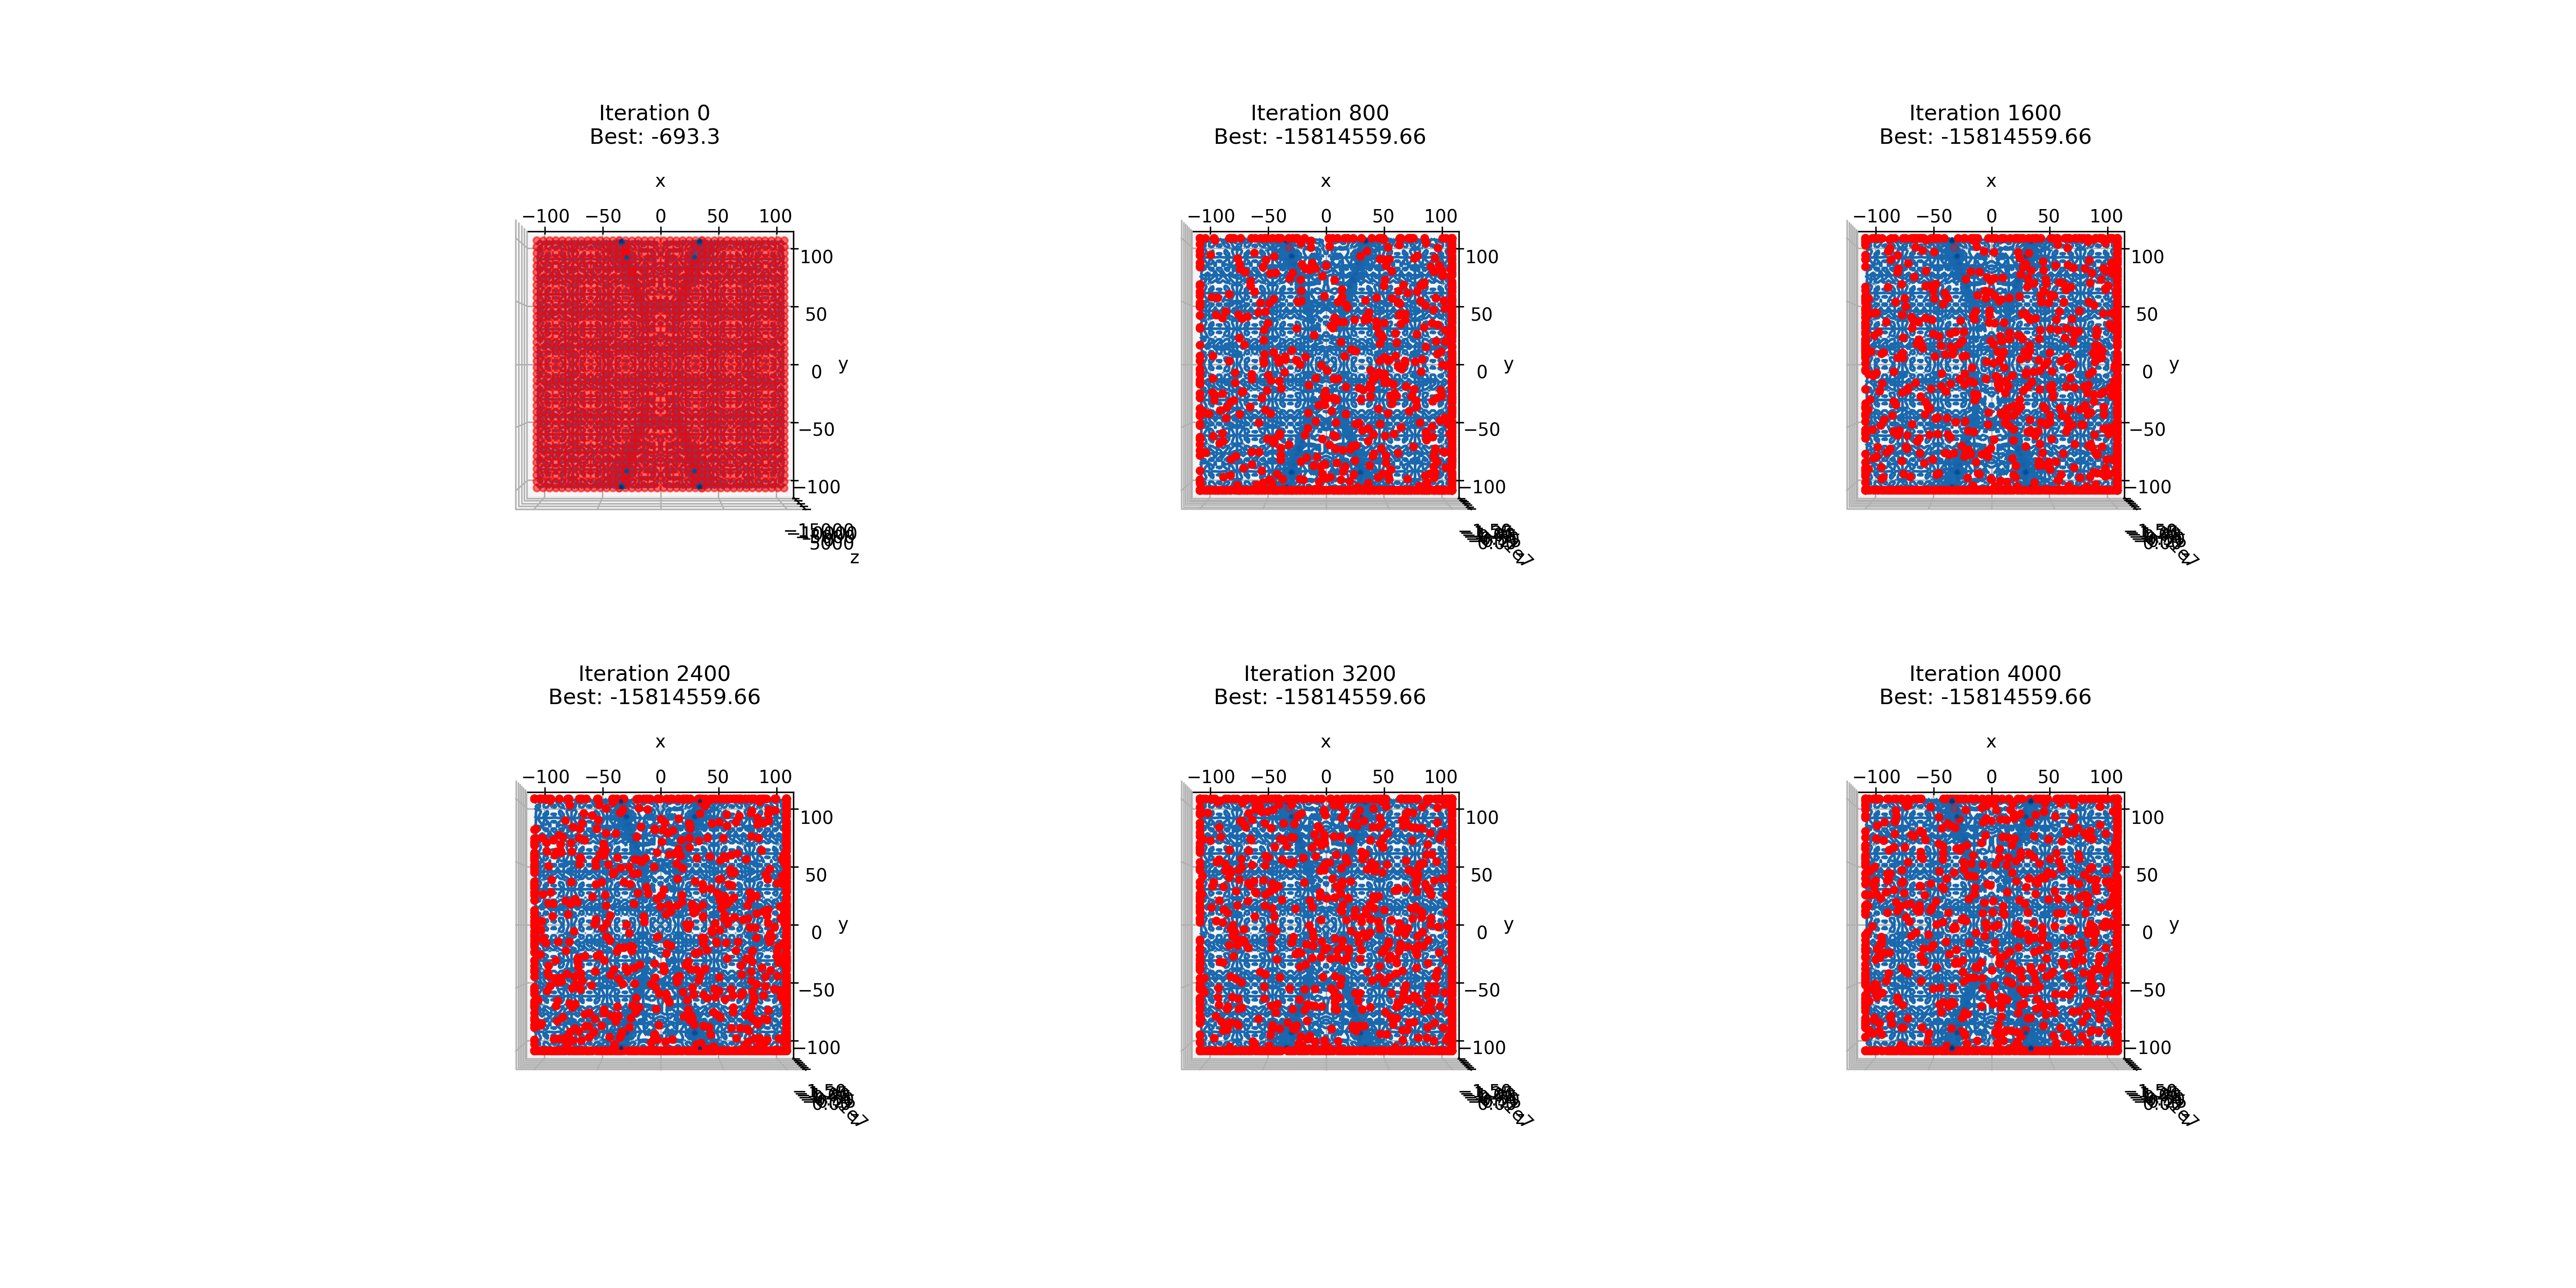
\includegraphics[width=1\textwidth]{results/g.png}
\end{center}

همانطور که دیده می‌شود ذرات هنوز همگرا نشده بودند اما با این وجود پاسخی در حدود
$-15 \times 10^6$
به دست آوردیم که چیزی حدود ۹ برابر بهتر از خواسته تمرین می‌باشد.


\end{document}
\LTR
\begin{lstlisting}[language=Python]
\end{lstlisting}
\RTL























ابتدا کلاس
\texttt{IO}
را پیاده‌سازی می‌کنیم که مسئله را از فایل ورودی خوانده و نتیجه را در فایل خروجی ذخیره کند.

\LTR
\begin{lstlisting}[language=Python]
class IO:
    @classmethod
    def init(cls, num):
        cls.num = num
        cls.o = open(f'output{cls.num}.stock', 'w')

    @classmethod
    def read(cls):
        with open(f'input{cls.num}.stock') as f:
            t = f.read()
        return t

    @classmethod
    def print(cls, t='', to_file=False):
        print(t)
        if to_file:
            cls.o.write(str(t) + '\n')
\end{lstlisting}
\RTL

در
\texttt{constructor}
این کلاس شماره مسئله را به عنوان ورودی دریافت می‌کنیم و فایل خروجی را باز می‌کنیم. همچنین متد
\texttt{read}
مسئله ورودی را خوانده و به صورت خام برمی‌گرداند. متد
\texttt{print}
نیز اطلاعات را روی
\texttt{iostream}
چاپ می‌کند. همچنین در صورتی که پارامتر دوم این متد
\texttt{True}
باشد اطلاعات را در فایل خروجی نیز وارد می‌کند. برای اطلاعات غیرضروری مانند جزئیات هر تکرار، این پارامتر را
\texttt{False}
در نظر می‌گیریم و تنها پاسخ نهایی مسئله را در فایل ذخیره می‌کنیم.

همچنین نیاز داریم تا پس از خواندن ورودی خام، آن را
\texttt{parse}
کنیم. این کار را به کمک قابلیت
\texttt{regex}
در پایتون انجام می‌دهیم.

\LTR
\begin{lstlisting}[language=Python]
# Read length and requests from input file
NUM = 5
IO.init(NUM)
raw_input = IO.read()
length = int(re.findall(r'Stock Length:\s*(\d+)', raw_input)[0])
requests = list(map(int, re.findall(r'Requests:((\s*\d+,)*\s*(\d+)?)', raw_input)[0][0].split(',')))
\end{lstlisting}
\RTL

\newpage
\section{کلاس تنه}
کلاسی برای نمایندگی تنه‌ها (کاغذ، تیرآهن، ...) در پایتون پیاده‌سازی می‌کنیم.

\LTR
\begin{lstlisting}[language=Python]
class Stock:
    def __init__(self, length=None):
        if length is not None:
            self.__free_length = length
            self.__cuts = []
    def copy(self):
        new = Stock()
        new.__free_length = self.__free_length
        new.__cuts = self.__cuts.copy()
        return new
\end{lstlisting}
\RTL

متد
\texttt{constructor}
این کلاس، به عنوان تنها ورودی طول را دریافت می‌کند. در هر
\texttt{instance}
از این کلاس، لیستی از برش‌های آن را، به همراه فضای خالی باقی‌مانده نگه می‌داریم. هرچند فضای خالی از روی برش‌ها و طول کل قابل محاسبه است اما به این روش هزینه محاسباتی کم‌تری متحول می‌شویم و در هر لحظه به فضای باقی‌مانده دسترسی داریم. همچنین متد
\texttt{copy}
را برای کپی کردن یک تنه پیاده‌سازی می‌کنیم. این متد زمانی که می‌خواهیم پاسخی در همسایگی یک پاسخ ایجاد کنیم کاربردی است چرا که نمی‌خواهیم پاسخ اصلی تغییری کند اما پاسخ جدیدی مانند آن با کمی تغییر ایجاد شود پس برای حل مشکل
\texttt{mutable}
بودن
\texttt{instance}ها
در پایتون به این متد نیاز خواهیم داشت. دو متد بسیار ساده
\texttt{add}
و
\texttt{remove}
را به این کلاس اضافه می‌کنیم. توجه کنیم که در هر متد لازم است همزمان به اضافه یا کم کردن یک برش به تنه، فضای آزاد را تغییر دهیم، و همچنین هنگام اضافه کردن برش دقت کنیم که فضای آزاد کافی وجود داشته باشد.

\LTR
\begin{lstlisting}[language=Python]
def add(self, length):
    if self.__free_length >= length:
        self.__free_length -= length
        self.__cuts.append(length)
    else:
        raise Exception('insufficient free length')
def remove(self, index):
    self.__free_length += self.__cuts[index]
    self.__cuts.remove(self.__cuts[index])
\end{lstlisting}
\RTL

متد ساده
\texttt{empty}
را نیز برای بررسی خالی بودن یک تنه اضافه می‌کنیم که تنه‌هایی که در طی جست‌وجو خالی می‌شوند را حذف کنیم و هنگامی که هزینه یک پاسخ را بر اساس تعداد تنه‌های آن پاسخ محاسبه می‌کنیم هزینه درستی بیابیم.

\LTR
\begin{lstlisting}[language=Python]
def empty(self):
    return not self.__cuts
\end{lstlisting}
\RTL

متدهای شناخته‌شده
\texttt{\_\_str\_\_}
و
\texttt{\_\_repr\_\_}
را نیز برای نمایش یک تنه پیاده‌سازی می‌کنیم که در فایل سورس موجود است.

\newpage
\section{پاسخ}
برای نمایندگی پاسخ‌های مسئله کلاسی به اسم
\texttt{Answer}
پیاده‌سازی می‌کنیم که مشخصا شامل لیستی از تنه‌ها می‌باشد. مقداردهی
\texttt{instance}های
این کلاس را به صورت تصادفی انجام می‌دهیم. به این صورت که لیست درخواست‌ها را در
\texttt{constructor}
به عنوان ورودی دریافت می‌کنیم و این لیست را بر می‌زنیم. سپس از ابتدا شروع می‌کنیم و تا جایی که ممکن است درخواست‌ها را به یک تنه اختصاص می‌دهیم و هر زمان که این کار ممکن نبود یک تنه جدید ایجاد می‌کنیم.

\LTR
\begin{lstlisting}[language=Python]
class Answer:
    def __init__(self, length=None, requests=None):
        if length is not None and requests is not None:
            self.length = length
            self.__stocks = []
            indexes = list(range(len(requests)))
            random.shuffle(indexes)
            for i in indexes:
                try:
                    self.__stocks[-1].add(requests[i])
                except:
                    self.__stocks.append(Stock(length))
                    self.__stocks[-1].add(requests[i])
    def copy(self):
        new = Answer()
        new.length = self.length
        new.__stocks = [stock.copy() for stock in self.__stocks]
        return new
\end{lstlisting}
\RTL

متد
\texttt{copy}
را نیز به برای ایجاد یک پاسخ مانند پاسخ فعلی اما با قابلیت تغییر ایجاد می‌کنیم. می‌بینیم که در اینجا از متد کپی که روی
\texttt{Stock}
تعریف شده بود استفاده کردیم.

متد ساده زیر نیز برای محاسبه هزینه هر پاسخ به کار می‌رود که برابر تعداد تنه‌های پاسخ می‌باشد.

\LTR
\begin{lstlisting}[language=Python]
def stocks_count(self):
    return len(self.__stocks)
\end{lstlisting}
\RTL

مشابه بخش قبل،  متدهای
\texttt{\_\_str\_\_}
و
\texttt{\_\_repr\_\_}
را نیز برای نمایش پیاده‌سازی می‌کنیم.

\LTR
\begin{lstlisting}[language=Python]
def __str__(self):
    return 'Number of Stocks: ' + str(self.stocks_count()) + '\n' + 'Stocks:\n' + ''.join(map(str, self.__stocks)) + '\n'

def __repr__(self):
    return self.__str__()
\end{lstlisting}
\RTL

\newpage
\section{جست‌وجو در همسایگی}
برای یافتن پاسخ‌های نزدیک به یک پاسخ، سعی می‌کنم یک برش تصادفی از یک تنه تصافی پاسخ انتخاب کنیم و آن را به یک تنه تصادفی دیگر منتقل کنیم. اما توجه کنیم که در این صورت هیچ‌گاه پاسخ بدتر نخواهد شد چرا که هزینه پاسخ برابر تعداد تنه‌های موجود در پاسخ است و در این صورت این تعداد هرگز بیشتر نخواهد شد لذا الگوریتم تبرید تدریجی بی‌معنی است و در واقع در حال پیاده‌سازی الگوریتم
\lr{\texttt{Hill Climbing}}
می‌باشیم.

برای حل این مشکل زمانی که می‌خواهیم یک برش را به یک تنه دیگر منتقل کنیم، با احتمال کمی، یک تنه جدید می‌سازیم. اگر فرض کنیم
$n$
تنه داریم، می‌توانیم یک تنه خالی به این لیست اضافه کنیم که در این صورت احتمال انتخاب این تنه در اردر
$\frac{1}{n}$
خواهد بود. پس با احتمال
$\frac{1}{n}$
یک تنه جدید ایجاد می‌کنیم و قطعه را در آن تنه قرار می‌دهیم و در غیر این صورت دو تا از تنه‌های موجود را برای انجام عملیات استفاده می‌کنیم.

از آنجا که تنها یک جابجایی تغییر بسزایی ایجاد نمی‌کند تعداد این جابجایی‌ها را عدد بزرگ‌تری انتخاب می‌کنیم تا قابلیت پویش را افزایش دهیم و فضای بیشتری در اطراف را مورد بررسی قرار دهیم. برای این منظور پارامتری به اسم
\texttt{MUTATION\_DEGREE}
در نظر می‌گیریم و هر بار عددی تصادفی بین ۱ و این پارامتر انتخاب می‌کنیم و آن قدر تلاش می‌کنیم یک برش را منتقل کنیم تا به این تعداد بار انتقال موفق انجام شود. (اگر تنه مقصد فضای خالی نداشته باشد برش ناموفق خواهد بود.)

پس متد
\texttt{mutate}
را برای کلاس
\texttt{Answer}
به صورت زیر تعریف می‌کنیم که پاسخی مشابه خودش خروجی می‌دهد با تعدادی جابجایی برش.

\LTR
\begin{lstlisting}[language=Python]
def mutate(self, degree):
    count = random.randint(1, degree)
    new = self.copy()
    while count > 0:
        if random.random() > 1 / self.stocks_count():
            stock_0, stock_1 = random.choices(new.__stocks, k=2)
        else:
            stock_0 = random.choice(new.__stocks)
            stock_1 = Stock(new.length)
            new.__stocks.append(stock_1)

        if stock_0.transfer_a_cut_to(stock_1):
            count -= 1
        if stock_0.empty():
            new.__stocks.remove(stock_0)
        if stock_1.empty():
            new.__stocks.remove(stock_1)
    return new
\end{lstlisting}
\RTL

توجه کنیم که در نهایت اگر تنه‌هایی که در آن‌ها تغییر ایجاد کردیم خالی شدند آن‌ها را حذف می‌کنیم.

می‌بینیم که در کد بالا از متد
\texttt{transfer\_a\_cut\_to}
بر روی کلاس
\texttt{Stock}
استفاده شده. این متد به صورت زیر پیاده‌سازی شده‌است.

\LTR
\begin{lstlisting}[language=Python]
def transfer_a_cut_to(self, other):
    cut_index = random.randrange(len(self.__cuts))
    try:
        other.add(self.__cuts[cut_index])
        self.remove(cut_index)
        return True
    except:
        return False
\end{lstlisting}
\RTL

\newpage
\section{فرار از رکود و بهینه‌های محلی}
در این تمرین از روشی ابتکاری به اسم
\texttt{chaos}
یا آشوب استفاده کردیم تا اگر در بهینه محلی گیر کردیم بتوانیم فرار کنیم. الگوریتم مشابه تبرید تدریجی کلاسیک پیاده‌سازی شده با این تفاوت که در هر تکرار الگوریتم، چنانچه پاسخ جدید مشابه پاسخ قبلی بود معیاری به اسم
\texttt{stagnancy}
را افزایش می‌دهیم که از همین معیار برای شرط توقف نیز استفاده می‌کنیم.

اما تفاوت این الگوریتم این است که در هر تکراری که در رکود می‌گذراند معیاری به اسم
\texttt{chaos}
را به میزان پارامتری به اسم
\texttt{CHAOS\_DEGREE}
افزایش می‌دهد. و این پارامتر را به عنوان ضریبی برای دما در نظر می‌گیرد. یعنی دما به صورت تدریجی کم می‌شود اما هرگاه در یک نقطه راکد شدیم، دما را به صورت تدریجی زیاد می‌کنیم (الزاما زیاد نمی‌کنیم، در بعضی موارد سرعت کم شدن کم می‌شود) به امید آن که با بالا نگه داشتن دما بتوانیم از بهینه محلی بگریزیم.

با توجه به مشاهدات، ایجاد آشوب در بعضی موارد به خصوص مسئله شماره ۵ بسیار موثر واقع شد و موفق شدیم بارها از بهینه محلی بگریزیم و نقاط بهتری پیدا کنیم. این ایده در طبیعت نیز وجود دارد که آشوب باعث بهینگی بیشتری در انتها می‌شود.

\newpage
\section{پیاده‌سازی}
کد پیاده‌سازی این الگوریتم به صورت زیر خواهد شد.

\LTR
\begin{lstlisting}[language=Python]
# Run the Simulated Annealing
start = time.time()
TEMPERATURE = lambda iteration, chaos: .99 ** (iteration / 100) * chaos
MUTATION_DEGREE = 5
STAGNANCY_THRESHOLD = 5000
CHAOS_DEGREE = .1

stagnancy = 0
current = Answer(length, requests)
best = current
last = current
iteration = 0
chaos = 1
while True:
    temperature = TEMPERATURE(iteration, chaos)
    IO.print(f'{iteration}\t{current.stocks_count()}\t{temperature}')
    iteration += 1
    new = current.mutate(MUTATION_DEGREE)
    delta = new.stocks_count() - current.stocks_count()
    if delta < 0 or random.random() < math.exp(-delta / temperature):
        current = new
    if last.stocks_count() == current.stocks_count():
        stagnancy += 1
        chaos += CHAOS_DEGREE
    else:
        stagnancy = 0
        chaos = 1
    if stagnancy > STAGNANCY_THRESHOLD:
        break
    last = current
    if current.stocks_count() < best.stocks_count():
        best = current

IO.print()
IO.print(best, True)
IO.print(f'Iterations: {iteration}', True)
IO.print(f'Time: {time.time() - start}', True)
IO.o.close()    
\end{lstlisting}
\RTL

\newpage
\section{بررسی نتایج}

\subsection{مسئله اول}
با اجرای الگوریتم در
\texttt{13.65}
ثانیه و پس از
\texttt{89706}
تکرار به پاسخ
\texttt{51}
می‌رسیم، جزئیات برش‌ها در فایل
\texttt{output1.stock}
موجود است.

\subsection{مسئله دوم}
با اجرای الگوریتم در
\texttt{13.56}
ثانیه و پس از
\texttt{90305}
تکرار به پاسخ
\texttt{78}
می‌رسیم، جزئیات برش‌ها در فایل
\texttt{output2.stock}
موجود است.

\subsection{مسئله سوم}
با اجرای الگوریتم در
\texttt{4.08}
ثانیه و پس از
\texttt{83447}
تکرار به پاسخ
\texttt{101}
می‌رسیم، جزئیات برش‌ها در فایل
\texttt{output3.stock}
موجود است.

\subsection{مسئله چهارم}
با اجرای الگوریتم در
\texttt{10.56}
ثانیه و پس از
\texttt{84112}
تکرار به پاسخ
\texttt{222}
می‌رسیم، جزئیات برش‌ها در فایل
\texttt{output4.stock}
موجود است.

\subsection{مسئله پنجم}
با اجرای الگوریتم در
\texttt{491.28}
ثانیه و پس از
\texttt{135750}
تکرار به پاسخ
\texttt{4325}
می‌رسیم، جزئیات برش‌ها در فایل
\texttt{output5.stock}
موجود است.

\end{document}
و
\texttt{train}
و همچنین کلاس‌های پیش‌بینی‌شده برای داده
\texttt{test}
قابل رؤیت است.

\subsection{تغییر تعداد لایه‌های مخفی}
کد زیر در فایل
\texttt{7.py}
موجود است. در این کد در یک حلقه، هر بار لایه‌های مخفی را متفاوت در نظر می‌گیریم. مانند موارد قبل برای سنجیدن مدل از داده‌های
\texttt{test}
به جای
\texttt{train}
استفاده می‌کنیم.

\LTR
\lstinputlisting[language=Python]{7.py}
\RTL

خروجی به صورت زیر خواهد شد.

\begin{center}
    \includegraphics[width=\textwidth]{figs/7.png}
\end{center}

همانطور که در تصویر قابل‌مشاهده است به نظر می‌رسد همان یک لایه مخفی با سه نورون بهتر از سایر حالات عمل می‌کند.
\end{document}